% Created 2023-03-05 Sun 19:02
% Intended LaTeX compiler: pdflatex
\documentclass[11pt]{article}
\usepackage[utf8]{inputenc}
\usepackage[T1]{fontenc}
\usepackage{graphicx}
\usepackage{longtable}
\usepackage{wrapfig}
\usepackage{rotating}
\usepackage[normalem]{ulem}
\usepackage{amsmath}
\usepackage{amssymb}
\usepackage{capt-of}
\usepackage{hyperref}
\usepackage{minted}
\usepackage[default]{sourcecodepro}
\usepackage[T1]{fontenc}
\usepackage[a4paper, total={6in, 8in}]{geometry}
\usepackage{lipsum}
\renewcommand{\contentsname}{Contenido}
\author{Diego Domínguez}
\date{\today}
\title{}
\hypersetup{
 pdfauthor={Diego Domínguez},
 pdftitle={},
 pdfkeywords={},
 pdfsubject={},
 pdfcreator={Emacs 28.2 (Org mode 9.6)}, 
 pdflang={English}}
\begin{document}

\tableofcontents \clearpage
\section{Explicación del programa}
\label{sec:orgdef71fa}
El programa incorpora un árbol de búsqueda binaria
(ABB) en \emph{C++}, haciendo uso de memoria dinámica
(apuntadores) y de manejo de archivos utilizando delimitadores.

Las operaciones codificadas para el árbol fueron:
\begin{itemize}
\item Insertar
\item Imprimir inorden
\item Imprimir posorden
\item Imprimir preorden
\item Eliminar nodo
\item Eliminar árbol
\item Buscar
\item Leer archivo
\item Guardar archivo
\item Salir
\end{itemize}

\section{Cómo se organizo el TDA}
\label{sec:orgffe1549}
El nodo que contiene el tipo de dato \emph{Student}
contiene tres atributos:
\begin{itemize}
\item name
\item age
\item major
\end{itemize}
Al insertar un nuevo nodo al árbol el programa
pedirá estos tres datos, añadiéndolos al final
como un solo tipo de dato (recuerdos de Datos 1).

\section{Estrategia de almacenamiendo y recuperación de datos}
\label{sec:orgf5ab984}
\section{Explicación de las funciones}
\label{sec:org0369fbe}
\subsection{Insertar}
\label{sec:org319dfca}
\begin{minted}[]{cpp}
void Tree::insert(Student data){
    if(root == nullptr){
        root = new TreeNode(data);
    }else{
        TreeNode* current = root;
        while(true){
            if(data.name < current->data.name){
                if(current->left == nullptr){
                    current->left = new TreeNode(data);
                    break;
                }else{
                    current = current->left;
                }
            }else{
                if(current->right == nullptr){
                    current->right = new TreeNode(data);
                    break;
                }else{
                    current = current->right;
                }
            }
        }
    }
    std::cout << "\nAlumno agregado" << std::endl;
}
\end{minted}
\begin{itemize}
\item Recibe el tipo de dato \emph{Student}
\item Devuelve el nodo \emph{root} si es el primer nodo
insertado en el árbol
\item Si no, recorre el árbol por la izquierda
comparando el dato \emph{name} con el nodo \emph{current}
hasta asignarlo
\item Si el nombre es ``mayor'', recorre por la derecha
hasta encontrar su lugar
\end{itemize}
\subsection{Imprimir inorden}
\label{sec:orgef47a5d}
\begin{minted}[]{cpp}
void Tree::traverseInOrder(TreeNode* node){
    if(node != nullptr){
        traverseInOrder(node->left);
        std::cout << node->data.name
                  << " ("
                  << node->data.age
                  << ", "
                  << node->data.major
                  << ")" << std::endl;
        traverseInOrder(node->right);
    }
}
\end{minted}
\begin{itemize}
\item Mientras el nodo sea distinto de nulo, recorre
la parte izquierda
\item Llegando al tope, imprime los datos del nodo visitado
\item Recorre la parte izquierda
\end{itemize}
\subsection{Imprimir posorden}
\label{sec:org241ae15}
\begin{minted}[]{cpp}
void Tree::traversePostOrder(TreeNode* node){
       if(node != nullptr){
               traversePostOrder(node->left);
               traversePostOrder(node->right);
               std::cout << node->data.name
                         << " ("
                         << node->data.age
                         << ", "
                         << node->data.major
                         << ")" << std::endl;
       }
}
\end{minted}
\begin{itemize}
\item Se mueve a la izquierda
\item Se mueve a la derecha
\item Llegando al tope, imprime el nodo visitado
\end{itemize}
\subsection{Imprimir preorden}
\label{sec:org4e82436}
\begin{minted}[]{cpp}
void Tree::traversePreOrder(TreeNode* node){
    if(node != nullptr){
            std::cout << node->data.name
                      << " ("
                      << node->data.age
                      << ", "
                      << node->data.major
                      << ")" << std::endl;
            traversePreOrder(node->left);
            traversePreOrder(node->right);
    }
}
\end{minted}
\begin{itemize}
\item Imprime el nodo visitado
\item Se mueve a la izquierda
\item Se mueve a la derecha
\end{itemize}
\subsection{Eliminar nodo}
\label{sec:org24022a7}
\begin{minted}[]{cpp}
void Tree::deleteNode(TreeNode* root, std::string& name){
    if (root == nullptr){
        return;
    }

    if(root->data.name == name){
        if(root->left == nullptr && root->right == nullptr){
            delete root;
            root = nullptr;
        }else if(root->left == nullptr){
            TreeNode* temp = root;
            root = root->right;
            temp->right = nullptr;
            delete temp;
        }else if(root->right == nullptr){
            TreeNode* temp = root;
            root = root->left;
            temp->left = nullptr;
            delete temp;
        }else{
            TreeNode* temp = root->right;
            while(temp->left != nullptr){
                temp = temp->left;
            }
            root->data.name = temp->data.name;
            deleteNode(root->right, temp->data.name);
        }
    }else if(name < root->data.name){
        deleteNode(root->left, name);
    }else{
        deleteNode(root->right, name);
    }
}
\end{minted}
\begin{itemize}
\item Busca el nodo a eliminar en el lado izquierdo y
derecho del árbol
\item Si el nodo es encontrado con el nombre específico
\begin{itemize}
\item Verifica si tiene un hijo, dos o ninguno
\begin{itemize}
\item Si tiene ninguno elimina el nodo
\item Si tiene uno, el padre del nodo visitado
apuntará al hijo del nodo, esté en la
izquierda o en la derecha
\item Si tiene dos, mientras el nodo sea distinto
de nulo, se recorre a la izquierda, moviendo
los datos a su consiguiente, y eliminando el
más a la derecha
\end{itemize}
\end{itemize}
\end{itemize}

\subsection{Eliminar árbol}
\label{sec:org3c49737}
\begin{minted}[]{cpp}
void Tree::deleteAll(TreeNode* root){
        if(root == nullptr){
                return;
        }

        deleteAll(root->left);
        deleteAll(root->right);

        delete root;
        root = nullptr;
}
\end{minted}
\begin{itemize}
\item Si el nodo es nulo, regresa
\item Si no, llama recursivamente al lado izquierdo
del nodo
\item Al igual que el derecho
\item Eliminando el nodo visitado
\item Para terminar aterrizándolo
\end{itemize}
\subsection{Buscar}
\label{sec:orgd1af7ef}
\begin{minted}[]{cpp}
void Tree::search(TreeNode* root, std::string name){
        if(root == nullptr){
                return;
        }
        search(root->left, name);
        if(root->data.name == name){
                std::cout << "Alumno encontrado:" << std::endl;
                std::cout << root->data.name
                        << ", " << root->data.age
                        << ", " << root->data.major << std::endl;
        }
        search(root->right, name);
}
\end{minted}
\begin{itemize}
\item Si el nodo es nulo, regresa, indicando que no se encontró
\item Si no, busca por la izquierda
\begin{itemize}
\item Si el nodo actual corresponde al nombre a
buscar, lo imprime
\end{itemize}
\item Si no, busca por la izquierda
\end{itemize}
\subsection{Leer archivo}
\label{sec:org34e97cd}
Utiliza dos funciones
\begin{minted}[]{cpp}
TreeNode* Tree::readFile(const std::string filename,
                         const char fDel, const char rDel){

        std::ifstream file;
        file.open(filename);

        TreeNode* root = nullptr;

        readFileHelper(root, file, fDel, rDel);

        std::cout << "Archivo leído" << std::endl;

        return root;
}
\end{minted}
Que simplemente abre el archivo con los parámetros
\emph{filename}, crea un nodo raíz y llama a
\emph{readFileHelper} con los delimitadores de campo y registro

Cabe aclarar que los delimitadores utilizados son:
\begin{itemize}
\item \textbf{,} para campos
\item \textbf{Carácter de salto de línea} para registros
\end{itemize}
Haciendo que el archivo \emph{file01.txt} termine de la
siguiente manera:
\begin{itemize}
\item Diego,21,Ingeniería
\item María,22,Contaduría
\item Naomi,21, Veterinaria
\end{itemize}
Continuando con la función \emph{readFileHelper}
\begin{minted}[]{cpp}
void Tree::readFileHelper(TreeNode*& node,
                    std::ifstream& file,
                    const char fDel,
                    const char rDel){

        std::string name;
        // Necesario para leerlo del archivo,
        // de ahí lo convertimos a int
        std::string ageStr;
        std::string major;

        getline(file, name, fDel);
        getline(file, ageStr, fDel);
        getline(file, major, rDel);

        if(name.empty() || ageStr.empty() || major.empty())
                node = nullptr;
        else{
                int age = stoi(ageStr);

                // Leemos de la misma manera en que leemos
                // el archivo
                node = new TreeNode(Student(name, age, major));
                readFileHelper(node->left, file, fDel, rDel);
                readFileHelper(node->right, file, fDel, rDel);
        }
}
\end{minted}
Se crean 3 variables para retomar los datos del
archivo
\begin{itemize}
\item name
\item ageStr
\item major
\end{itemize}
Siendo todos \emph{string}, a pesar que \emph{age} debería
ser \emph{int}, el archivo de texto no lo reconoce como
entero, por lo tanto, es necesario cambiarlo a su
dato correspondiente en memoria.

\begin{itemize}
\item Verifica si uno de los campos está vacío (por si
pasa lo peor), y crea el nodo en vacío.
\item Si no, hace el cambio a \emph{int} para la variable \emph{age}
\item Crea un nuevo nodo con todos los datos obtenidos
\item Llama a la función del lado izquierdo y derecho
\end{itemize}
La forma en la que lee el archivo es de la misma
manera en la que la impresión preorden, ¡importante
para poder tener los datos en orden!
\subsection{Guardar archivo}
\label{sec:org5e9d1f2}
De la misma manera para leer el archivo, la forma
que guarda es en dos funciones
\begin{minted}[]{cpp}
bool Tree::saveFile(TreeNode* root, const std::string& filename,
                    const char fDel, const char rDel){

        std::ofstream file;
        file.open(filename);

        saveFileHelper(root, file, fDel, rDel);

        file.close();
        // Para changes, false para saber que no hay
        // changes, jeje, ¿entiendes?
        return false;
}
\end{minted}
\begin{itemize}
\item Crea un archivo con el nombre específicado
\item Llama a
\end{itemize}
\begin{minted}[]{cpp}
void Tree::saveFileHelper(TreeNode* node, std::ofstream& file,
                          const char fDel, const char rDel){

        if(node == nullptr){
                return;
        }

        // Recorrido preorden PREORDEN
        // Guarda el nodo
        // Se va al izquierdo y derecho
        file << node->data.name << fDel
                << node->data.age << fDel
                << node->data.major << rDel;

        saveFileHelper(node->left, file, fDel, rDel);
        saveFileHelper(node->right, file, fDel, rDel);
}
\end{minted}
\begin{itemize}
\item Añade cada uno de los datos conforme a los
delimitadores de campo y registro mencionados
\item Llama a la función por la derecha y por la izquierda
\end{itemize}
\subsection{Salir}
\label{sec:orgc856224}
Digo, es\ldots{}intuitivo, ¿no?

\begin{minted}[]{cpp}
        do{
                option = choose();
                switch(option){
                        // Insertar
                        case '1':{
                                readInput();
                                oak.insert(Student(student.name,
                                                   student.age,
                                                   student.major));
                                break;
                        }
                        // Inorden
                        case '2':{
                                if(oak.isTreeEmpty(oak.root))
                                        std::cout << "No existe" << std::endl;
                                else{
                                        std::cout << &oak.root << std::endl;
                                        shoutItOut();
                                        oak.traverseInOrder();
                                }
                                break;
                        }
                        // Posorden
                        case '3':{
                                if(oak.isTreeEmpty(oak.root))
                                        std::cout << "No existe" << std::endl;
                                else{
                                        shoutItOut();
                                        oak.traversePostOrder();
                                }
                                break;
                        }
                        // Preorden
                        case '4':{
                                if(oak.isTreeEmpty(oak.root))
                                        std::cout << "No existe" << std::endl;
                                else{
                                        shoutItOut();
                                        oak.traversePreOrder();
                                }
                                break;
                        }
                        // Eliminar nodo
                        case '5':{
                                std::string lookfor;
                                std::cin.ignore();
                                std::cout << "Nombre a eliminar: ";
                                getline(std::cin, lookfor);
                                oak.deleteNode(oak.root, lookfor);
                                break;
                        }
                        // Eliminar árbol
                        case '6':{
                                oak.deleteAll(oak.root);
                                oak.root = nullptr;
                                break;
                        }
                        // Buscar
                        case '7':{
                                std::cin.ignore();
                                std::string lookfor;
                                std::cout << "Nombre a buscar: ";
                                getline(std::cin, lookfor);
                                oak.search(oak.root, lookfor);
                                break;
                        }
                        // Leer archivo
                        case '8':{
                                // Haz que elimine lo que está
                                // anteriormente para así no gastar
                                // memoria
                                oak.root = oak.readFile(filename, fDel, rDel);
                                break;
                        }
                        // Guardar archivo
                        case '9':{
                                char subOption;
                                if(!oak.isFileEmpty(filename)){
                                        std::cout << "El archivo tiene "
                                                << "contenido, "
                                                << "¿sobreescribir?\n"
                                                << "1. Sí 2. No: ";
                                        std::cin >> subOption;
                                        switch(subOption){
                                            case '1':{
                                                    changes = oak.saveFile(oak.root,
                                                                           filename,
                                                                           fDel,
                                                                           rDel);
                                                    break;
                                            }
                                            case '2':{
                                                    std::cout << "Saliendo"
                                                              << std::endl;
                                                    break;
                                            }
                                            default:
                                                    std::cout << "Inválido,"
                                                              << "saliendo"
                                                              << std::endl;
                                            }

                                }else{
                                        changes = oak.saveFile(oak.root,
                                                               filename,
                                                               fDel,
                                                               rDel);
                                }
                                break;
                        }
                        case 'S':{
                                std::cout << "Adiós" << std::endl;
                                break;
                        }
                        case 's':{
                                std::cout << "Adiós" << std::endl;
                                break;
                        }
                        default:
                                std::cout << "Opción incorrecta" << std::endl;
                }

        }while(option != 's' && option != 'S');
\end{minted}

Tanto código para una función sencilla que no cabe
en el documento.
Es el menú en el main, la opción de salida es \emph{s}.
\section{Capturas de pantalla}
\label{sec:org0352024}
Programa recién abierto
\begin{center}
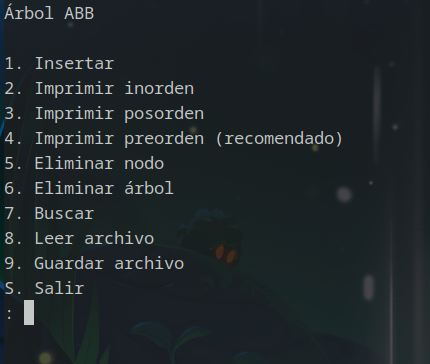
\includegraphics[width=.9\linewidth]{./principal.png}
\end{center}

Insertando un dato
\begin{center}
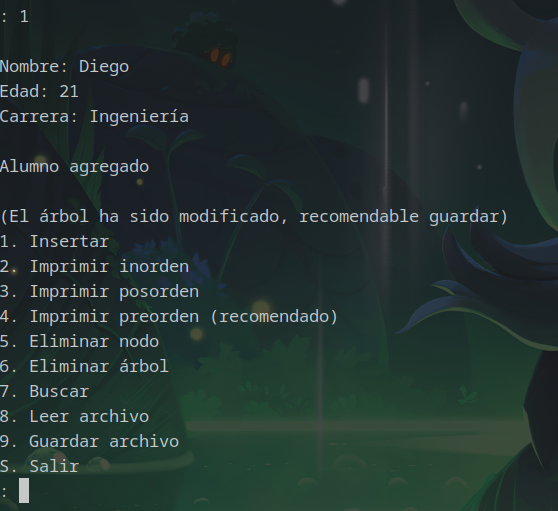
\includegraphics[width=.9\linewidth]{./insertando.png}
\end{center}
El programa muestra si se modificó el árbol

Imprimiendo los datos
\begin{center}
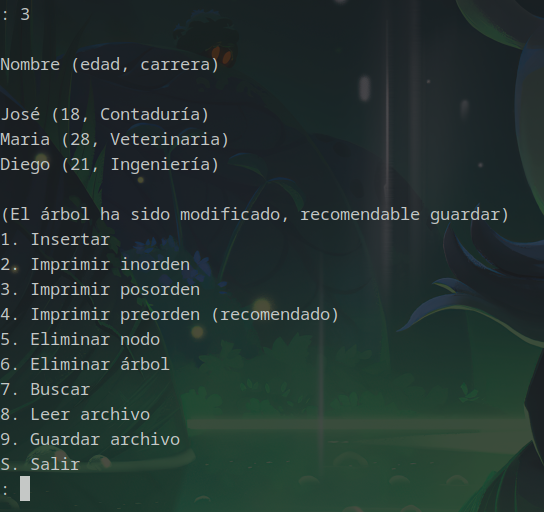
\includegraphics[width=.9\linewidth]{./imprimiendo.png}
\end{center}

Guardando a archivo
\begin{center}
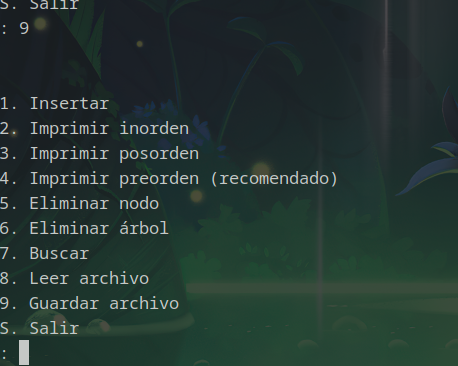
\includegraphics[width=.9\linewidth]{./guardando.png}
\end{center}


Mostranddo el archivo guardado, mostrando los
campos separados por los delimitadores previamente
mencionados
\begin{center}
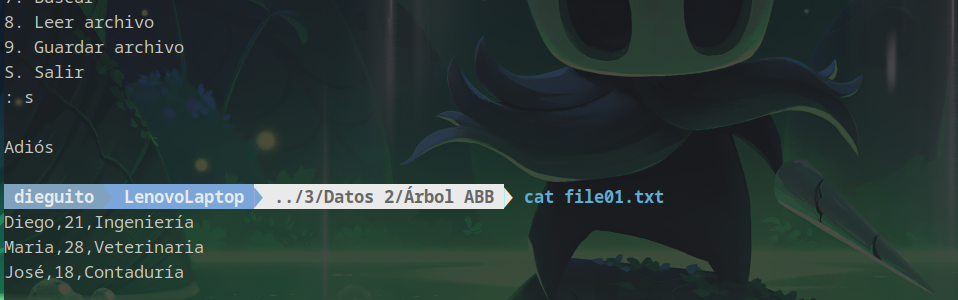
\includegraphics[width=.9\linewidth]{./mostrando.png}
\end{center}

Reabriendo el archivo y cargándolo a memoria
\begin{center}
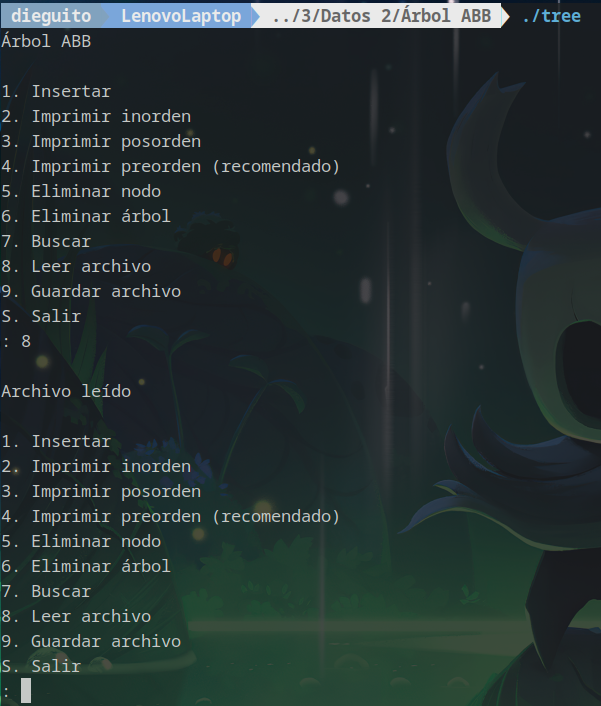
\includegraphics[width=.9\linewidth]{./reabriendo.png}
\end{center}

Mostrando que sí se guardó
\begin{center}
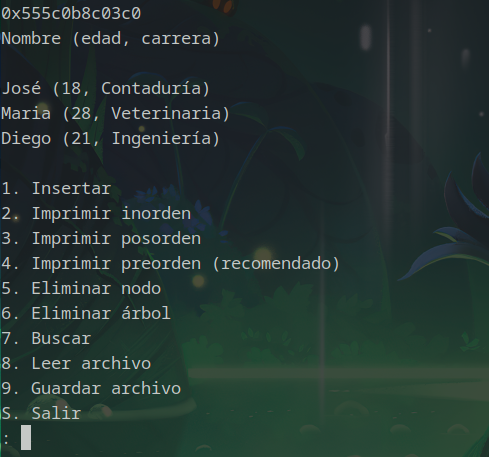
\includegraphics[width=.9\linewidth]{./reimprimiendo.png}
\end{center}

\section{Conclusiones}
\label{sec:org314505b}
Me partí el coco intentando entender los árboles,
no tengo más opinión sobre esto, esperando a los
grafos con miedo.
\end{document}